\documentclass[12pt]{article}
\usepackage{geometry}
\geometry{letterpaper, left=22.5mm, right=22.5mm, top=30mm, bottom=30mm}
\geometry{letterpaper}
\usepackage{amsmath}
\usepackage{amssymb}
\usepackage{enumitem}
\usepackage{fancyhdr}
\usepackage{framed}
\usepackage{tikz}
\usepackage{mathpazo}
%\usepackage{charter}
%\usepackage{newcent}
\usepackage{indentfirst}
\usepackage{booktabs}
\usepackage{graphicx}
\usepackage{float}
\usepackage{makecell}
\usepackage{xcolor}
\usepackage{mdframed}
\usetikzlibrary{trees}
\pagestyle{fancy}
\usepackage{amsthm}
\theoremstyle{definition}
\newtheorem{definition}{Definition}[section]
\theoremstyle{property}
\newtheorem{property}{Property}[section]
\theoremstyle{assumption}
\newtheorem{assumption}{Assumption}[section]
\theoremstyle{example}
\newtheorem{example}{Example}[section]
\theoremstyle{comment}
\newtheorem{comment}{Comment}[section]
\newtheorem{theorem}{Theorem}[section]
\newtheorem{corollary}{Corollary}[theorem]
\newtheorem{lemma}[theorem]{Lemma}
\usepackage{lastpage}
\usepackage{wrapfig}
\usepackage{hyperref}
\usepackage{subcaption}
\usepackage{setspace}
\hypersetup{
colorlinks=true,
linkcolor=black,
filecolor=green, 
urlcolor=blue,
}
\newcommand{\ROM}[1]
    {\MakeUppercase{\romannumeral #1}}
    
    \DeclareMathOperator*{\plim}{plim}
\fancyhead[L]{Econometrics \ROM{2}: Recitation 12}%change each reci
\fancyhead[R]{Spring 2022}
\fancyfoot[C]{\thepage \hspace{1pt} / \pageref{LastPage}}

\fancypagestyle{firstpage}{%
\fancyhf{}%
\renewcommand{\headrulewidth}{0mm}%
  \fancyfoot[C]{\thepage \hspace{1pt} / \pageref{LastPage}}
}
%change title each rec
\title{Introduction to Econometrics \ROM{2}: Recitation 12}

\begin{document}
\linespread{1.25}
\onehalfspacing

\author{Seung-hun Lee\footnote{Contact me at \href{mailto:sl4436@columbia.edu}{sl4436@columbia.edu} if you spot any errors or have suggestions on improving this note.}}
\date{April 25th, 2022}
\maketitle
\thispagestyle{firstpage}

%%%%%%%%%%%%%%%%%%

\section{Regression Discontinuity}
In some cases, finding an instrumental variable $Z_i$ that satisfies relevance, exclusion, and monotonicity might be difficult. To avoid comparison being contaminated by selection bias, one idea is to compare the entities that barely made the treatment against those who barely missed out. This might be easier if the explicit cutoff for being treated is known - think about a means-tested social program, distance, winning margin, or test score cutoffs. The comparison assumes that these individuals around the cutoff are otherwise equal and thus the treatment assignment is as good as random.  This approach that leverages discontinuities in treatment assignment is called \textbf{regression discontinuity design} (commonly abbreviated to RD or RDD). \par
Regression discontinuity approach actually started from Psychology in 1960s and was brought into the mainstream of applied economics very recently. Whenever you learn applied microeconomics class in your second year, you are bound to read or present about a paper that uses this research design. \par
As its name suggests, this approach exploits the discontinuities in the treatment assignment. So the key difference between regression discontinuity and previous frameworks is that RDD does not require the overlap condition in the sense that $p(X_i)\in(0,1)$. In fact, one of the design has $p(X_i)=1$ for $X_i\geq c$ and $0$ otherwise. Another thing that RDD should satisfy is that for every other covariates, the distribution should remain continuous even through the discontinuity, so that entities around the cutoff are observationally equal except for treatment assignment.\par


\subsection{Regression discontinuity: Setup and framework}
We will start with a \textbf{sharp RDD}. You can think of this case as a case where the assignment into the treatment is determined by
\[
D_i=\mathbb{1}(Z_i\geq c(W_i))
\]
where $Z_i$ is a running (forcing) variable determining cutoffs, $c(W_i)$ can be a known function of $W_i$ or just a constant. In this setup, everyone who is eligible under the cutoff rules are treated, and those that are ineligible are left out of the treatment. We also keep the potential outcome framework from before, but we will slightly change this to
\begin{align*}
y_i& = D_iy_i(1)+(1-D_i)y_i(0)\\
&=y_i(0)+D_i(y_i(1)-y_i(0))\\
&=y_i(0)+\mathbb{1}(Z_i\geq c(W_i))\cdot(y_i(1)-y_i(0))
\end{align*}
We also keep the regressional framework for the potential outcomes, $y_i(d)=\mu(W_i,Z_i,d)+\epsilon_i(d)$. One key assumption that we will carry through this section is the continuity of the conditional expectation on potential outcomes at $Z_i=c(W_i)$
\begin{mdframed}[backgroundcolor=blue!5] 
\begin{assumption}[Continuity of $\mu(W_i,Z_i,d)$ at $Z_i=c$] If $Z_i$ has a known cutoff at $c$, we assume that $E[y_i(1)|W_i, Z_i]$ and $E[y_i(0)|W_i, Z_i]$ are continuous around $Z_i=c$. Put if differently, 
\[
E[y_i(d)|W_i, Z_i=c^+]=E[y_i(d)|W_i, Z_i=c^-] \  \text{for each } d\in\{0,1\}
\]
This also implies that the distribution of $(\mu_i(W_i, Z_i,0),\mu(W_i, Z_i,1))$ and $(\epsilon_i(0),\epsilon_i(1))$ is continuous at $Z_i=c$
\end{assumption}
\end{mdframed}\par
This is to ensure that those who are treated and untreated are observationally equivalent, at least around the cutoff (and a very local area). If this condition is not satisfied, this implies that there could be more than the $Z_i$ variable that jumps around the cutoff, which may lead to incorrect estimate of the treatment effect or tendencies to bunch at the cutoff to join the treatment (manipulation). This can be formally tested with McCrary test or visually.   \par
There is another version of the RDD which is more general than the sharp RDD. A \textbf{fuzzy RDD} setup exploits the jump in the probability of being treated at $Z_i=c(W_i)$. This jump is not necessarily from 0 to 1. Intuitively, this is a case where not all of the eligible entities are treated, or if there is an ineligible participant under the cutoff rules that are treated (or both). Formally, we say we look for discontinuities of 
\[
\Pr(D_i|W_i,Z_i)
\]
at $Z_i=c(W_i)$. Sharp RDD can be thought of as a very special case of fuzzy RDD.  
\subsection{Identification with regression discontinuity}
 Assume that $c(Z_i)$ is a constant $c$. We can write
\begin{align*}
E[y_i|W_i, Z_i]&=E[y_i(0)|W_i, Z_i]+E[(y_i(1)-y_i(0))\mathbb{1}(Z_i\geq c)|W_i, Z_i]
\end{align*}
And we can separate the above into two. One with $Z_i=c^+$ and the other with $Z_i=c^-$.
\begin{align*}
E[y_i|W_i, Z_i=c^+]&=E[y_i(0)|W_i, Z_i=c^+]+E[y_i(1)-y_i(0)|W_i, Z_i=c^+]\\
E[y_i|W_i, Z_i=c^-]&=E[y_i(0)|W_i, Z_i=c^-]
\end{align*}
This is because $1(Z_i\geq c(W_i))=1$ if $Z_i=c^+$ and 0 otherwise. Therefore, 
\begin{align*}
E[y_i|W_i, Z_i=c^+] - E[y_i|W_i, Z_i=c^-]&=E[y_i(0)|W_i, Z_i=c^+]-E[y_i(0)|W_i, Z_i=c^-]\\
 &\ \ \ \ +E[(y_i(1)-y_i(0))|W_i, Z_i=c^+]\\
 &=E[(y_i(1)-y_i(0))|W_i, Z_i=c^+]
\end{align*}
where $E[y_i(0)|W_i, Z_i=c^+]-E[y_i(0)|W_i, Z_i=c^-]=0$ due to the continuity assumption. Reusing the continuity argument that $E[y_i(d)|W_i, Z_i=c^+]=E[y_i(d)|W_i, Z_i=c^-] \ \text{for each } d\in\{0,1\}$, we can write  
\[
E[y_i(1)-y_i(0)|W_i, Z_i=c^+]=E[y_i(1)-y_i(0)|W_i, Z_i=c]
\]
Therefore, we have backed out
\[
E[y_i(1)-y_i(0)|W_i, Z_i=c]=E[y_i|W_i, Z_i=c^+] - E[y_i|W_i, Z_i=c^-]
\]
which is the average treatment effect at $Z_i=c$ and a given $W_i$. The remaining questions is to determine the range of $c^+$ and $c^-$. To gain internal validity, we select a narrow bandwidth around the cutoff $[c-h, c+h]$ that optimized the tradeoff between bias and variance. Narrower bands will increase accuracy at the expense of volatility. Higher bandwidths may lead us to oversmoothe, leading to less variance but more bias. We will talk about bandwidths in the next section.\par
We can say very little about those outside of the cutoff. Moreover, since those far above the cutoff maybe significantly different from those far below, such comparison may not be very well explained with an RDD framework. Therefore, RDD designs in generla have very little external validity. \par
This is similar to the LATE in the sense if we let $\mathbb{1}(Z_i\geq c)$ be an IV for participation, we can get back what is effectively equivalent to the LATE estimator, with the difference in the probability of treatment exactly at 1. Also, we are looking at the treatment effect on the compliers, albeit a very narrow group of people. Lastly, like LATE, RDD estimates tell us very little about those who are not within the narrow bandwidth of our cutoff and the extrapolation to explain the other groups are tricky. 
\par
For a Fuzzy RDD, the identification is done as follows
\begin{align*}
E[y_i|W_i, Z_i]&=E[y_i(0)|W_i, Z_i]+E[(y_i(1)-y_i(0))\Pr(D_i=1|W_i, Z_i)|W_i, z_i]
\end{align*}
So we can do the similar approach as in sharp RDD and get 
\footnotesize{\begin{align*}
E[y_i|W_i=w, Z_i=c^+]&=E[y_i(0)|W_i=w, Z_i=c^+]+\Pr(D_i=1|W_i=w, Z_i=c^+)E[y_i(1)-y_i(0)|W_i=w, Z_i=c^+]\\
E[y_i|W_i=w, Z_i=c^-]&=E[y_i(0)|W_i=w, Z_i=c^-]+\Pr(D_i=1|W_i=w, Z_i=c^-)E[y_i(1)-y_i(0)|W_i=w, Z_i=c^-]
\end{align*}}\normalsize
So using the continuity assumption, the difference in the left hand side can be written as
\footnotesize{\begin{align*}
E[y_i|W_i=w, Z_i=c^+]-E[y_i|W_i=w, Z_i=c^-]&=[\Pr(D_i=1|W_i=w, Z_i=c^+)-\Pr(D_i=1|W_i=w, Z_i=c^-)]\\
&\ \ \ \ \times E[y_i(1)-y_i(0)|W_i=w, Z_i=c]
\end{align*}}\normalsize
Thus, we also identify an average treatment effect at $Z_i=c$ and $W_i=w$, which is now divided by something that is not necessarily 1. 
\[
E[y_i(1)-y_i(0)|W_i=w, Z_i=c]=\frac{E[y_i|W_i=w, Z_i=c^+]-E[y_i|W_i=w, Z_i=c^-]}{\Pr(D_i=1|W_i=w, Z_i=c^+)-\Pr(D_i=1|W_i=w, Z_i=c^-)}
\]


\subsection{Implementing regression discontinuity}
So what can we do in terms of implementing the RDD in practice? One way to implement RDD in practice is to make use of nonparametric regression. The bandwidth, however, should be bounded at $c$. If you are doing a nonparametric regression from the left of the bandwidth, you should apply this on $[c-h, c)$. For the right hand side, $[c, c+h]$. If the domain reaches beyond $c$ from either side, there is a huge risk of misfitting the data. While you can do local constant regression in theory, it comes at a huge cost. With this, you can only pin down the level of $y_i$ from either side. You lose out the rate in which outcome changes within both sides of the boundary. Therefore, if carrying out nonparametric regression, you should do at least a local linear regression. \par
Since we are doing a nonparametric regression, we also run into similar problems as in the typical nonparametric regressions. If you have many other variables to consider, you risk running into the curse of dimensionality. There is also an issue of selecting an optimal bandwidth. We still minimize the MSE, but at $Z_i=c$.  $MSE(h)$ is defined as 
\[
E[(\hat{\mu}(w,c,0)-\mu(w,c,0))^2+(\hat{\mu}(w,c,1)-\mu(w,c,1))^2]
\]
Calonico, Cattaneo, and Tituinik (2014) suggests the use of local quadratic estimator with the optimal bandwidth selected by minimizing above $MSE(h)$ which is typically known as IK bandwidth (Imbens, Kalyanaraman, 2012). Also note that the same trade-off between variance and bias is still in play. \par
There is also a parametric way to implement this as well. One way is to run a separate regression for both left and right of the cutoff. That is, run
\begin{gather*}
y_i = W_i\beta^- +(c-Z_i)W_i\gamma^-+\epsilon_i^-\ \ \text{for }Z_i<c\\
y_i = W_i\beta^+ +(Z_i-c)W_i\gamma^++\epsilon_i^+\ \ \text{for }Z_i\geq c
\end{gather*}
This setup allows us to fit a different trend on the left and the right of the cutoff $c$. There is also a way in which we make use of both sides of the cutoff. Specifically, we run
\[
y_i = W_i\beta+ W_i \cdot 1(Z_i\geq c)\gamma+W_i\cdot(c-Z_i)\delta+W_i\cdot (c-Z_i)\cdot 1(Z_i\geq c) \mu +\epsilon_i
\]
Here, what happens is that
\begin{itemize}
\item $Z_i\geq c$: $y_i=W_i(\beta+\gamma)+W_i\cdot(c-Z_i)(\delta+\mu)$
\item $Z_i< c$: $y_i=W_i(\beta)+W_i\cdot(c-Z_i)(\delta)$
\end{itemize}
To make this simple, suppose that $W_i$ is just a vector of 1's. Then, on the $(y_i, Z_i)$ plane,  the jump of the outcome at $Z_i=c$ would be captured by the $\gamma$ parameter. Using $\delta, \mu$, we can allow the slopes to differ on either side of the equation. However, setting up parametrically relies on a possibly extreme form of extrapolation. So whenever nonparametric estimation is feasible, it is highly recommended to do so. \par
There are some graphical tests that should be carried out. First, we plot $y_i$ as a function of $Z_i$ for a given $W_i$ and see if there is a mean shift. Also, we plot the propensity score $\Pr(D_i=1|W_i, Z_i)$ and look for a shift. One thing that should not shift is the distribution of $W_i$'s. So plot $W_i$'s as function of $Z_i$ and confirm that there is no shift. Another thing to worry regarding $Z_i$ is the possibility of manipulating or gaming. Maybe it might be possible to get into the treatment when you should not be treated (e.g. Ost et al. (2018) checks for this). Therefore, use a McCrary test to confirm that the distribution of $W_i$ do not change at $Z_i=c$. \par
Last but not least, what if we do not know the exact cutoff? That is actually not much to worry about, since we can figure out what they might be based on the distribution of $Z_i$. Chay, McEwan, and Urquiola (2005) conducts and RDD in the context where the exact cutoffs are unknown using visual evidence. Also, since we lose a lot of data in selecting the optimal bandwidth around the cutoff, RDD is usually poor in terms of external validity.


\subsection{Presenting regression discontinuity as design}
Regression discontinuity outcome is usually presented visually through graphs - one with the running variable $Z_i$ and the treatment status $D_i$ to check jumps in propensity score. The other set of graphs contain the $Z_i$ and all other covariates $W_i$ to see if treated and the untreated are observationally equal around the cut off. The last set of graphs plots $y_i$ onto $Z_i$ to see if the outcome jumps around the cutoff. For instance, if we are in the public finance context and study the effect of a particular welfare program with a means-tested benefit assignment mechanism, we could use the means-tested criteria as our $Z_i$. If we are to study the effect of a specific educational program offered to those below a particular test score, that score could be the $Z_i$. Here are some works that deal use RDD. 

\begin{mdframed}[backgroundcolor=yellow!5] 
\begin{example}[Lee, JoE 2008] This paper focuses on the elections won and lost by a very narrow margin. The logic is that in such case, winning and losing is effectively randomized. The running variable is the Democrat vote share $-$ Republican vote share. Key finding is that Democrats who barely win an election are much more likely to run for office and succeed in the next election, compared to Democrats who barely lost. In general this paper finds positive relationship between margin of victory and electoral outcomes and identifies an incumbent advantage. 
\end{example}


\begin{example}[Howell, AER 2017] This paper assess the impact of R\&D subsidies from the government to new ventures. The rank on the application to the R\&D is used as a running variable (a discrete running variable, thus typical McCrary test is infeasible).  The paper finds that an early-stage award approximately doubles the probability that a firm receives subsequent venture capital (summarized in the figure below) and has large, positive impacts on patenting and revenue. These effects are stronger for more financially constrained firms.

\begin{figure}[H]
\centering
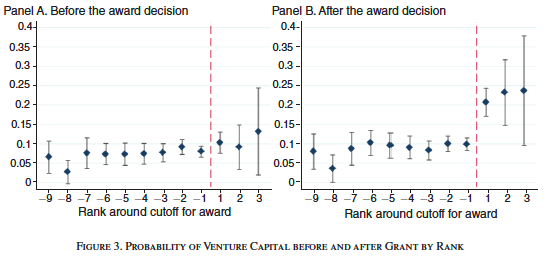
\includegraphics[width=0.6\textwidth, keepaspectratio]{RD_fig.png}
\caption{Reception of venture capital, before and after}
\end{figure}
\end{example}
\begin{example}[Dell, ECMA 2010] This paper uses RDD to examine the long-run impacts of the extractive institutions (forced labor, or mita) in Peru and Bolivia in 1573-1812 period. Results indicate a prevalence of stunted growth in children and drop in household consumption in affected districts today. Areas subject to mita had few large landowners and lower education attainment, among other mechanisms. Cutoff is based on the borders of the communities which differ in latitude and longitude, thus \textbf{multidimensional}. Subjected communities had to send 1/7 of adult males to work in mines, while communities out of the border were exempt.
\begin{figure}[H]
\centering
\includegraphics[width=0.7\textwidth, keepaspectratio]{RD_Dell.png}
\caption{Consumption and Stunting (Darker: less consumption and more stunting)}
\end{figure}
\end{example}
\end{mdframed}

\section{Machine Learning}
Machine learning in the context of econometrics is interested in model selection for prediction - finding the parsimonious model in the context of a very large dataset. Underlying tradeoff here is that increasing the fit of the model to the data, which is a focus of conventional statistics, reduces bias but leads to overfitting issues that increases variance in the prediction. Therefore, there is a serious interest in finding an optimal specification that is compact and minimizes prediction errors. It ranges from regularized models such as LASSO, Ridge regression, and elastic nets and methods that are much more involved - random forests and neural networks. All of them differ in how they fine-tune the model. \par
\subsection{Model Selection}
Often, we are interested in controlling a large set of covariates (e.g. propensity score). We can generalize this to the structure where structure refers to specification as well as parameter values. In determining the structure, we face a trade-off: We are tempted to increase the number of covariates since it allows us to fit the data better. However, in doing so, we risk overfitting - the out-sample prediction can perform poorly in terms of variance. Therefore, some method to penalize complexity is required. 
\par
We start with a set $\mathcal{M}$ of candidate models. Then for a model $M\in\mathcal{M}$, we define a penalty parameter $p(M)$ that increases in complexity (think of the number of coefficients). Two classical information criteria include
\begin{itemize}
\item Akaike's Information Criterion: Choose $M$ satisfying
\[
\min_{M}\left(\min_\theta\left[ -\sum_{i=1}^n \log{l_i(\theta;M)}+2p(M) \right]\right)
\]
\item Bayesian Information Criterion: Choose $M$ satisfying
\[
\min_{M}\left(\min_\theta\left[ -\sum_{i=1}^n \log{l_i(\theta;M)}+p(M)\frac{\log{n}}{2} \right]\right)
\]
\end{itemize}
The subtle difference between the two is that BIC tends to be harsher for complexities. This can be seen since for $\log{n}$ increases with $n$. Moreover, the derivation of BIC is based on a Bayesian probabilistic framework - If a selection of candidate models includes a true model for the dataset, then the probability that BIC selects the correct model approaches to 1 as training sample size increases (From Hastie, Tibshirani, Friedman "The Element of Statistical Learning", 2016). Therefore, BIC performs better for selecting the model within the given sample. For out-sample performance, AIC performs better. Both of them, however, can be impractical to calculate when we work with large models. This can be common especially if we allow for multiple levels of interaction between the covariates. In other words, if $p$ is a number of potential covariates, and $n$ is the sample size, we run into the case where $p>>n$. \par
One way out is to penalize complexities with the convex norm penalties. Define
\[
\Vert \theta \Vert _m = \sqrt[m]{\sum_{k=1}^p \vert \theta_k \vert ^m}
\]
and for $m=0$, we have $\Vert \theta \Vert _p=p$, penalties for the two information criteria above. Depending on the selection of $m$, we get different estimators that incorporates different shrinkage mechanisms - Ridge for $m=2$ and LASSO for $m=1$. \par
The general idea of shrinkage is as follows: We know that OLS is BLUE - It has the least variance among the linear, unbiased estimators. But what if we are willing to relax the 'unbiased' condition? Then can we find some estimators that have lower variance and even a lower mean squared error? James, Stein (1961) shows that it is possible and generalizable. \par 
Ridge and LASSO builds upon this idea, but uses different regularization methods. Consider the setup $Y_i=X_i\theta_0+\epsilon_i$. Ridge regression minimizes
\[
\sum_{i=1}^n(Y_i-X_i\theta_0)^2+\lambda\sum_{k=1}^p \theta_k^2 \ \ \left(\sum_{k=1}^p \theta_k^2=\Vert \theta\Vert_2^2\right)
\]
and yields
\[
\hat{\theta} = (X'X+\lambda I_p)^{-1}X'y
\]
Note that as $\lambda$ increases, the $(X'X+\lambda I_p)^{-1}$ term decreases, which drives the coefficients close to 0 and reduce overfitting. With LASSO, the minimization is 
\[
\frac{1}{n}\sum_{i=1}^n(Y_i-X_i\theta_0)^2+\lambda\sum_{k=1}^p |\theta_k| 
\] 
\par 
So what is the difference between LASSO and Ridge? Ridge regression drives your coefficients towards 0 but not equal to it. So when it comes to model selection in terms of ruling out irrelevant variables, LASSO does better. As far as computation is concerned, Ridge has a quicker computation speed and works relatively better with multicollinearity.  So the choice of the estimation method depends on your goal of minimizing MSE as well as computation power (but with modern computational power, LASSO is preferred to Ridge). \par
So what is the optimal $\lambda$? It depends on your goal. If your goal is to minimize the prediction error, you can use the following cross-validation methods to come up with one
\begin{itemize}
\item Leave-one-out: Leave one observation out at a time
\item Training vs Test sample: You split the sample into two, build a model given some $\lambda$ and gain prediction error from the test sample. Then, select $\lambda$ minimizing the prediction error there.
\item $K$-fold cross validation:  For $K-1$ blocks, estimate the model given some $\lambda$ and compute the error on the remaining block. Get this for $K$ blocks and compute the average error. Select $\lambda$ minimizing the error. 
\end{itemize}
\subsection{Decision-tree based models}

\subsubsection{Gradient descent methods}
Gradient descent refers to a first-order iterative optimization algorithm for finding the local minima of a function (for local maxima, we use gradient ascent). In our context, we want to minimize a loss function
\[
L(\theta) = \frac{1}{n}\sum_{i=1}^n l(y_i,\theta)
\]
where $l(\cdot)$ is continuously differentiable in $\theta$. Iteration is done by moving in the direction of a steepest descent (specified by the negative gradient) from the starting point. This process is repeated until the minima is reached. \par
Classical method of descent is based on Newton technique. Let's work with a scalar variable to get better ideas.  Note that the Taylor expansion of $L(\theta)$ around $\tilde{\theta}$ is
\[
L(\theta) \simeq L(\tilde{\theta})+L'(\tilde{\theta})(\theta-\tilde{\theta})+\frac{1}{2}L''(\tilde{\theta})(\theta-\tilde{\theta})^2
\]
Think of $\tilde{\theta}$ as our current point, $\theta^{(k)}$, and $\theta$ as the next point to be reached in our descent, $\theta^{(k+1)}$. We find the next point that minimizes the above approximation. In other words, we solve
\[
\frac{d}{d(\theta-\tilde{\theta})} = L'(\tilde{\theta}) + L''(\tilde{\theta})(\theta-\tilde{\theta})=0
\]
If we think of $\theta-\tilde{\theta}$ as the distance to move to the next point, we can see that it satisfies
\[
\theta= \tilde{\theta}-\frac{L'(\tilde{\theta})}{L''(\tilde{\theta})} \implies \theta^{(k+1)}= \theta^{(k)}-\frac{L'(\theta^{(k)})}{L''(\theta^{(k)})}
\]
If we take it to multiple dimensions, we can write $\theta^{(k+1)}= \theta^{(k)}-s_k \nabla L(\theta^{(k)})$ where $s_k$ is a sequence that converges to the inverse of a Hessian matrix at a minimum and $\nabla L(\cdot)$ is a gradient matrix. 
\par
While the idea itself is simple, implementation is difficult when we have large $n$ and $\theta$. With increasing dimensions and observations, we end up doing many more iterations, which can be costly. As an alternative, we can do a stochastic gradient method. The idea is to pick a random mini batch of $m$ observations, denoted as $B_k$ and use the estimate of a gradient from this set of observations to optimize (hence the name stochastic). In equation, 
\[
\theta^{(k+1)}= \theta^{(k)}-s_k \frac{1}{m}\sum_{i\in B_k} \nabla_\theta l (y_i, \theta^{(k)})
\]
where $\frac{1}{m}\sum_{i\in B_k} \nabla_\theta l (y_i, \theta^{(k)})$ is the average gradient. The additional noise (from using an estimated gradient instead of actual) is good for avoiding local minima that is far away from global minima, which can be potentially serious in high dimensional setups. The step size $s_k$ decreases as we approach the correct global minima and it is known to give an error in $\frac{1}{\sqrt{k}}$. \par
Another method is known as mini-batch gradient descent. It splits the training data into several mini-batches and conducts the optimization on each batch iteratively. The idea is to find a minimizer in the first batch $\theta^{(1)}$ from the first batch. Then use $\theta^{(1)}$ as a starting point and use the gradient descent in batch 2 to find a minimal in $\theta^{(2)}$. Repeat the process until the learning process slows down and we reach a global minima. \par
Stochastic gradient approach is a popular algorithm for training wide range of models in machine learning. It is the backbone of training artificial neural networks, alongside with back-propagation algorithm. Its use is reported in Geophysics and training of linear regression models in machine learning context. 

\subsubsection{Ensemble method}
Ensemble method combines multiple learning algorithms (think of regressions or decision trees) to obtain an algorithm with a better predictive performance that could be obtained from a single constituent learning algorithm alone. Think of ensemble as an average of predictions from multiple sources, with weights determined depending on the performance of the individual algorithms. Mathematically speaking, we choose weights $p_1,...,p_q$, where $q$ is the number of individual algorithms in use, that solves the following minimization problem 
\begin{gather*}
\min_{p_1,..,p_q}L\left( y, \sum_{m=1}^q p_m\hat{y}_m\right) \leq \min_{m\in\{1,..,q\}}L(y,\hat{y}_m)\\
\text{s.t.} \sum_{m=1}^q p_m=1, \ \ p_m\geq0
\end{gather*}
where $y$ is the target, or output of the algorithm, $p_m$ is the weight on algorithm $m$, and $\hat{y}_m$ is the prediction from algorithm $m$. The inequality may be strict when algorithms are different from each other significantly. 
\par
With the improvement in computing, there are many areas where this can be applied. In finance, it can be used to aid decision-making such as predicting financial crises, and detecting stock price manipulation\footnote{Kim, Sohn. 2012 ``Stock fraud detection using peer group analysis", \textit{Expert Systems with Applications}}. It is also used in remote sensing that studies land covers - from identifying land cover objects to detecting changes in them\footnote{Rodriguez-Galiano et al. 2012 ``An assessment of the effectiveness of a random forest classifier for land-cover classification", \textit{ISPRS Journal of Photogrammetry and Remote Sensing}}.


\subsubsection{Boosting}
Gradient boosting tries to reduce prediction errors in an iterative method starting from the weak learners - which can be understood as regression with few covariates and decision trees with few branches. It comes from ensemble approach in the sense that it combines the weak learners to get better prediction models. Our goal is to minimize the prediction error $\sum_{i=1}^n (y_i-\hat{y}_i)^2 $ from the simple models in class $\mathcal{M}$, while penalizing complexity. 
\par
We start with a null predictor $\hat{y}_i^{(0)}=0$ and residuals $r_i^{(0)}=y_i-\hat{y}_i^{(0)}=y_i$. Then we follow these steps:
\begin{enumerate}
\item Fit a sample model to the data $(x_i, r_i^{(0)} =y_i)$, penalize complexity, and get new predictors $\hat{r}_i^{(1)}$
\item Update the predictions $\hat{y}_i^{(1)}=\hat{y}_i^{(0)}+s\hat{r}_i^{(1)}$
\item Update the residuals $\hat{r}_i^{(1)}=\hat{r}_i^{(0)}-s\hat{r}_i^{(1)}$
\item Iterate for each $b=1,...,B$
\end{enumerate} \par
So how do we conduct the first step to get new predictors? In case of parametric models, let's say that there are such models $M$ with complexity penalty $p(M)$. Then, what we do is to choose $M$ and $\theta_M$ that minimizes
\[
\sum_{i=1}^n (r_i^{(b-1)}-r_M(x_i,\theta_M))^2+p(M)
\]
where $\hat{r}^{(b)}=r_M(x_i,\theta_M)$\par
Gradient boosting is used in any fields are the machines are trained to learn to rank (also known as machine-learned ranking). Some search engines are known to use this method to rank how the search order appears.  Some physics fields, such as high energy physics, uses this in their data analysis. 
%%%%%%%%%%%%%%%
\end{document}

